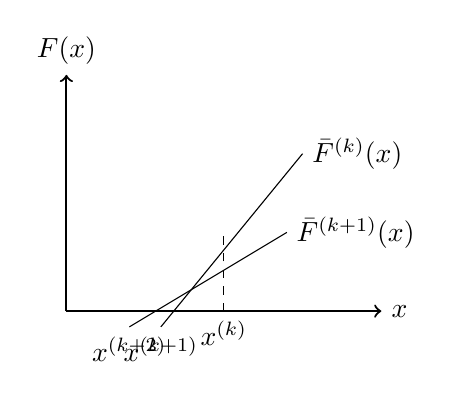
\begin{tikzpicture}
	\draw[thick,->] (0,0) -- (4,0) node[right]{$x$};
	\draw[thick,->] (0,0) -- (0,3) node[above]{$F(x)$};
	
	\draw (0.8, -0.2) node [below] {$x^{(k+2)}$} -- (2.8, 1) node [right] {$\bar{F}^{(k+1)}(x)$};
	\draw (1.2, -0.2) node [below] {$x^{(k+1)}$} -- (3, 2) node [right] {$\bar{F}^{(k)}(x)$};
	
	\draw [dashed] (2, 0) node [below] {$x^{(k)}$} -- ++(0,1);	
\end{tikzpicture} 
